% !TEX root = Bachelorarbeit.tex
\section{The seL4 Microkernel}\label{sec:seL4}
	The seL4 \cite{Manual} ist a small operation system kernel developed for the ARM11 arcitecture. All concepts, however, can be generalised to any architecture with a multilevel-page-table structure. \cite{PhDseL4} It is based on the L4 microkernel developed in the 1990s and proviedes a minimal number of services to applications, such as abstractions for virutal address spaces, threads, inter process comunication (IPC). \\
	Each abstraction ist implemented by a kernel object with methods dependent on the abstraction it supplies. If an application whants to use one of the implemented services it to call the corresponding object through capabilities. They are stored in kernel objects called \textit{CNodes}. \\
	Each capability contains a target object and potentially several access rights. The access rights can be \texttt{Read, Write, Grant} and \texttt{Create}. By invoking a capability that points to the kernel object  with a corresponding method name, applications can invoke system calls. As arguments these system calls can have data or other capabilities. For example: If an object has a capability with write authority in it, pointing on a synchronous endpoint, it can send a message to another object, that has read authority on this endboint. It can do it by invoking the capability, with the write right in it, that points on the synchronous endpoint object. The other object in turn has to own and invoke a capability with the read right in it, that also point on the synchronous endpoint.

\subsection{System Calls}
The kernel provides the following system calls:
\begin{itemize}
\item \texttt{send()}: The system call argument is delivered to the target object and the application is allowed to continue. If the target is not able to receive and/or process the arguments immediately, the sending application will be blocked until the arguments can be delivered.

\item \texttt{NBSend()}: Like \texttt{send()}. Exception: If the message is not deliverable it is silently droped.
\item \texttt{Call()}: Like \texttt{send()} but the application is blocked until the object provides a response, or the receiving application replies. \\
If the argument is delivered to an application via Endpoint the receiver needs the right to respond to the sender. So in this case an additional capability is added to the arguments. 
\item \texttt{Wait()}: If the target object is not ready \texttt{Wait()} is used by an application to block until the object is ready. 
\item \texttt{Reply()}: Used to respond to a \texttt{Call()}, using the capability generated by the \texttt{Call()} operation.
\item \texttt{ReplyWait()}: As a combination of \texttt{Reply()} and \texttt{Wait()} it is efficent for the common case that replying to a request and waiting for the next can be performed in a single system call. 
\end{itemize}
	
\subsection{Kernel Objects}\label{sec:KernelObjects}
The kernel implements several objects to allocate the system operations \cite{Manual}.
\begin{itemize}
\item \textbf{CNodes} \\
The capabilities to invoke system calls are stored in \textbf{\textit{CNodes}}. When created they get a fixed numer of slots that can be empty or contain a capability. 
The kernel constructs a \textbf{Capability Derivation Tree} (CDT) to keep records about the created capabilities and their associations. This is required for the revoke operation. \\ 
They have the following operations:
\begin{itemize}
\item \texttt{Mint()} \\
creates a copy of an existing capability. The new capability is placed in a specified CNode slot and may have less rights than the parent capability. In the CDT the capability is placed as child of the original one. 
\item \texttt{Copy()} \\
is similar to the Mint operation. But the new capability has the same rights as the original one and in the CDT it is represented as a sibling of it. 
\item \texttt{Move()} \\
can move a capability between two specified slots. 
\item \texttt{Mutate()} \\
moves the capability similar to \texttt{Move()} and is able to reduce its rights as it is done in \texttt{Mint()} without an orignal copy remaining.
\item \texttt{Rotate()} \\
moves two capabilities between three slots. Replaces two \texttt{Move()} operations. 
\item \texttt{Delete()} \\
can remove a capability from a specified slot.
\item \texttt{Revoke()} \\
is used to remove a complete part of the CDT. From a defined capability on, all children from the capability in the CDT are removed with \texttt{Delete()}. 
\item \texttt{Recycle()} \\
revokes all outstanding capabilities and reconfigures the object to its initial state. So the object can be reused in for another purpose.
\end{itemize}

\item \textbf{IPC Endpoints} \\
Endpoints are used for the \textit{interprocess communication} between threads. They can be devided into \textbf{synchronous (EP)} and \textbf{asynchronous (AEP)} endpoints. 
Threads in the seL4 kernel are grouped into security domains. Interprocess communication between different domains is only realised via AEPs. Generally capabilities to endpoints can be restricted to be read - or write - only. 
\item \textbf{TCP} \\
A thread of execution in seL4 is represented by a \textit{thread control block}. It is always associated with a CSpace (provides the capabilities required to manipulate the kernel objects) and a VSpace (provides the virtual memory environment required to contain the code and data application). \\
The thread control block object has the following methods: \\
\texttt{CopyRegisters(), ReadRegisters(), WriteRegisters(), SetPriority(), \\ SetIPCBuffer(), SetSpace(), Configure(), Suspend(), Resume()}
\item \textbf{Virtual Memory}\\
In the \textit{virtual address space} (VSpace) Objects in the VSpace implement services for the management of virtual memory which largely directly correspond to those of the hardware: \\
\begin{itemize}
\item seL4 ASID Table: \\
The seL4 \textit{Adress Space Identifier} table provides two services:
\begin{enumerate}
\item With the seL4 ASID table address spaces where mappings have to be removed from can easily be detected, as the seL4 acts as an internal naming mechanism for them.
\item In the seL4 PageDirectorys can be deleted without updating the capability links because the kernel sets the corresponding PageDirectory address in the ASID table to \textit{NULL} if a PageDirectory is revoked. Therefore the seL4 ASID table provied so called \textit{weak links} between capabilities on addresses in the ASID table and the VSpace mappings that are derived from them.
\end{enumerate}
The seL4 ASID table is a global, fixed-sized table that is created at boot time. Each seL4 ASID is associated with a hardware ASID.
\item PageDirectory (PD): \\
It defines the root page table of the two-level , hardware defined page table structure the ARM11 consists of. If an entity owns a authorised capability that points to a PD it has the right to manipulate the related VSpace.
\item PageTable (PT): \\
The leaf node of the ARM11, two-level page table structure is implemented by the PageTable object. A page table entry contains either an invalid
entry, or a pointer to a 4 kilobyte Page.
\item Pages or Frames: \\
A virtual memory page is implemented by region of physical memory called a \textit{Page} or \textit{Frame}. The name differs from paper to paper. In the specification it is called a \textit{Page} \cite{sel4}. It has three methods:
\begin{itemize}
\item If it gets an PD or PT capability as an argument the \texttt{map} installs a PD-entry or PT-entry and refers to the Page in the specified location.
\item If the permissions of an existing mapping have to be changed the Page calls the \texttt{remap} method.
\item The \texttt{unmap} method is used to remove an existing mapping.
\end{itemize}
\end{itemize}
The following illustrates the creation of a VSpace:
\begin{enumerate}
\item First a PD object has to be allocated with the retype operation on untyped memory objects. 
\item The \textit{Resource Manager} has to initialise it with a seL4 ASID table:
\begin{itemize}
\item It invokes the PD object
\item It passes a capability that allows the use of a slot in the seL4 ASID table. The memory address of the PD is copied into the provided ASID table slot. 
\item The capability pinting on the PD is updated by storing the sel4 ASID table index into it instead of the PD index. 
\end{itemize}
\item Now the PD can be used as a VSpace of one or more threads.
\item The ressource manager can install a PageTable into  an adress space by invoking a PageDirectory and passing a PageTable capability and the virtual address. After installing a PageTable the kernle stores the seL4 AID of the corresponding PD and the virtual address in the PT capability. 
\item With Pages the kernel proceed in a similar way. 
\end{enumerate}
Figure \ref{fig:intapp} shows how the objects of a VSpace are connected.
\begin{figure}[H]
	\centering
		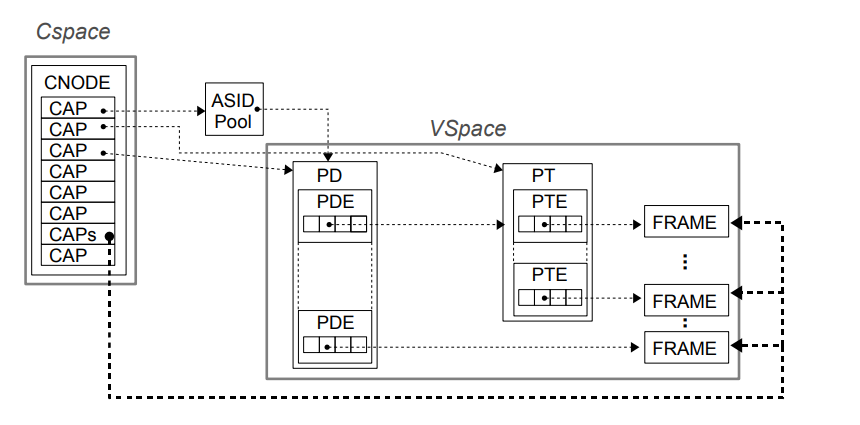
\includegraphics[width=0.7\textwidth]{./Pictures/applicationIntern.png}
	\caption[Internal representation of an application]{Internal representation of an application in seL4 \cite{sel4}}
	\label{fig:intapp}
\end{figure}
\item \textbf{Interrupt Objects} \\
Device driver applications require \texttt{Interrupt Ojects} to be capable of receiving and acknowledging interrupts from hardware devices.
\item \textbf{Untyped Memory} \\
\texttt{Untyped memory objects (UMO)} encapsulate a fixed-sized, size-aligned, continuous region of the physical memory. Each object can be devided into a group of smaller untyped memory objects. With \texttt{Retype()} a number of new kernel objects are created. It also returns capabilities to the new objects if it succeeds. 
\end{itemize}

\subsection{Memory Allocation Model} 
A special characteristic of the seL4 is that the memory for kernel objects is not allocated dynamically. A goal was to isolate physical memory access between applications and to control the amount of physical memory that applications can use. \\
To accomplish this applications get fixed sized memory regions they have to control by themselves. \\
Capabilities on Untyped Memory Objects (UMO) are needed to create new objects. So applications need the capabilities on UMOs to create new objects. After creation the objects have a fixed amount of memory they can use. \\
At boot time the kernel pre-allocates all the memory required for the kernel to run. This includes the space for kernel code, data and kernel stack. The kernel then creates an \textit{Initial User Thread} with associated CSpace and VSpace and hands over the remainig memory in form of capabilities on UMOs. \\
The Initial User Thread can create smaller sized UMOs out of an UMO or \texttt{retype} it into another object type. The creator of new objects has full authority over the objects. This "full authority" depends on the object type. \\
Figure \ref{fig:systarch} shows a sample system architecture in which a resource manager running at user-level  has the authority over the remaining untyped memory after bootstrapping. 
	
	\begin{figure}[ht]
	\centering
		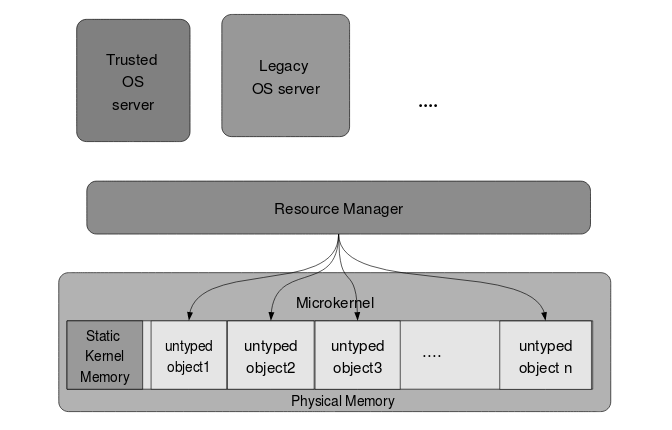
\includegraphics[width=0.6\textwidth]{./Pictures/MemoryAllocation.png}
	\caption[Sample system architecture]{Sample system configuration \cite{TakeG}}
	\label{fig:systarch}
	\end{figure}	